% EXPRESSsuite capabilities deck for ISO TC 184/SC 4 users.
% Build: pdflatex expresssuite-capabilities.tex (twice), then
%   pdftoppm -png -r 200 expresssuite-capabilities.pdf page
% and assemble the .pptx with docs/build-capabilities-pptx.py.
% Layout rules: Beamer 11pt on the default 4:3 frame, assertion headlines,
% nothing smaller than \footnotesize, about 60-100 words per slide.
\documentclass[11pt]{beamer}
\usepackage[T1]{fontenc}
\usepackage[utf8]{inputenc}
\usepackage{lmodern}
\usepackage{helvet}
\renewcommand{\familydefault}{\sfdefault}
\usepackage{listings}
\usepackage{booktabs}
\usepackage{array}
\usepackage{xcolor}
\usepackage{tikz}
\usepackage{graphicx}
\usetikzlibrary{arrows.meta,positioning}

\usetheme{default}
\useinnertheme{rectangles}
\definecolor{sc4blue}{RGB}{0,76,128}
\definecolor{sc4grey}{RGB}{90,90,90}
\definecolor{okgreen}{RGB}{0,110,60}
\definecolor{errred}{RGB}{170,30,30}
\setbeamercolor{structure}{fg=sc4blue}
\setbeamercolor{frametitle}{fg=sc4blue}
\setbeamerfont{frametitle}{size=\large,series=\bfseries}
\setbeamertemplate{navigation symbols}{}
\setbeamertemplate{footline}{%
  \begin{beamercolorbox}[wd=\paperwidth,ht=2.4ex,dp=1.2ex,leftskip=0.4cm,rightskip=0.4cm]{footline}
    \scriptsize\color{sc4grey}EXPRESSsuite 0.5.0 \quad \insertsection \hfill \insertframenumber/\inserttotalframenumber
  \end{beamercolorbox}}
\setbeamertemplate{itemize items}[circle]
\setlength{\leftmargini}{1.2em}
\setbeamertemplate{section page}{%
  \vfill\centering
  {\footnotesize\color{sc4grey}Section \insertsectionnumber}\\[0.6em]
  {\Large\bfseries\color{sc4blue}\insertsection}
  \vfill}
\AtBeginSection{\begin{frame}\sectionpage\end{frame}}

\lstdefinelanguage{EXPRESS}{
  morekeywords={SCHEMA,END_SCHEMA,ENTITY,END_ENTITY,TYPE,END_TYPE,SUBTYPE,OF,SUPERTYPE,ABSTRACT,SELF,WHERE,DERIVE,INVERSE,UNIQUE,USE,FROM,REFERENCE,LIST,SET,BAG,ARRAY,INTEGER,REAL,STRING,BOOLEAN,LOGICAL,NUMBER,ENUMERATION,EXTENSIBLE,BASED_ON,WITH,SELECT,GENERIC_ENTITY,RULE,END_RULE,FOR,FUNCTION,END_FUNCTION,RETURN,QUERY,EXISTS,SIZEOF,TYPEOF,IN,AND,OR,NOT,OPTIONAL},
  sensitive=false,
  morecomment=[l]{--},
  morecomment=[s]{(*}{*)},
  morestring=[b]',
}
\lstset{
  language=EXPRESS,
  basicstyle=\footnotesize\ttfamily,
  keywordstyle=\color{sc4blue}\bfseries,
  commentstyle=\color{sc4grey}\itshape,
  stringstyle=\color{okgreen},
  columns=fullflexible,
  keepspaces=true,
  showstringspaces=false,
  xleftmargin=0.6em,
  frame=none,
}
\newcommand{\diag}[1]{\par\medskip\noindent{\footnotesize\color{errred}\ttfamily #1}\par}
\newcommand{\code}[1]{\texttt{#1}}

\title{EXPRESSsuite}
\subtitle{A Visual Studio Code Insiders extension for EXPRESS schemas}
\author{For STEP developers and model reviewers}
\date{November 2026\\[0.5em]{\normalsize Software version 0.5.0}}

\begin{document}

\begin{frame}
  \titlepage
\end{frame}

\begin{frame}{The generic authoring loop: edit and check in VS Code, verify outside it, then commit}
  \centering
  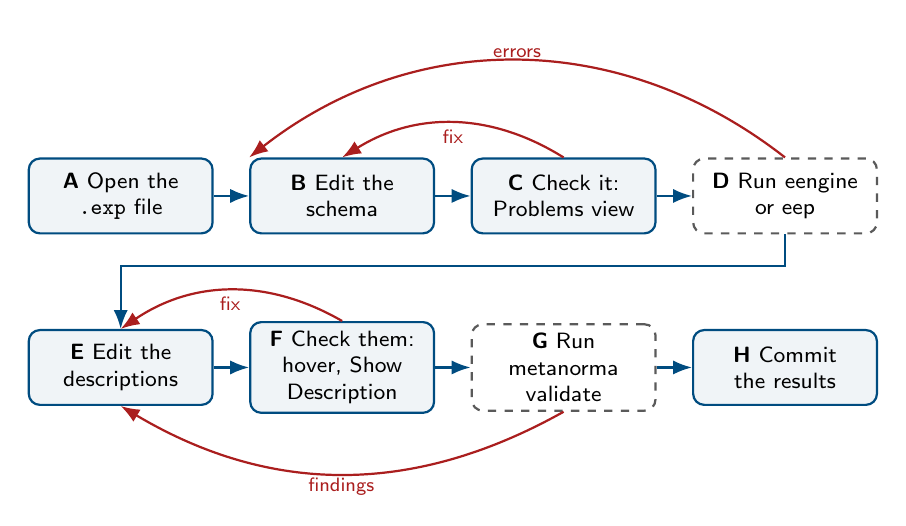
\begin{tikzpicture}[
      vsbox/.style={draw=sc4blue,thick,rounded corners,minimum height=0.95cm,text width=2.1cm,align=center,font=\footnotesize,fill=sc4blue!6},
      extbox/.style={draw=sc4grey,thick,dashed,rounded corners,minimum height=0.95cm,text width=2.1cm,align=center,font=\footnotesize},
      flow/.style={-{Latex[length=2.4mm]},thick,sc4blue},
      back/.style={-{Latex[length=2.4mm]},thick,errred},
      lab/.style={font=\scriptsize,color=errred,inner sep=1pt},
      node distance=0.45cm]
    % row 1: the schema
    \node[vsbox] (A) {\textbf{A} Open the \code{.exp} file};
    \node[vsbox,right=of A] (B) {\textbf{B} Edit the schema};
    \node[vsbox,right=of B] (C) {\textbf{C} Check it: Problems view};
    \node[extbox,right=of C] (T1) {\textbf{D} Run eengine or eep};
    % row 2: the descriptions
    \node[vsbox,below=1.2cm of A] (E) {\textbf{E} Edit the descriptions};
    \node[vsbox,right=of E] (F) {\textbf{F} Check them: hover, Show Description};
    \node[extbox,right=of F] (T2) {\textbf{G} Run metanorma validate};
    \node[vsbox,right=of T2] (H) {\textbf{H} Commit the results};
    % forward flow
    \draw[flow] (A) -- (B); \draw[flow] (B) -- (C); \draw[flow] (C) -- (T1);
    \draw[flow] (T1.south) -- ++(0,-0.4) -| (E.north);
    \draw[flow] (E) -- (F); \draw[flow] (F) -- (T2); \draw[flow] (T2) -- (H);
    % level-1 loops: a check sends you back one step
    \draw[back] (C.north) to[bend right=32] node[lab,below=1pt] {fix} (B.north);
    \draw[back] (F.north) to[bend right=32] node[lab,below=1pt] {fix} (E.north);
    % level-2 loops: an outside tool sends you back to editing
    \draw[back] (T1.north) to[bend right=38] node[lab,above] {errors} (B.north west);
    \draw[back] (T2.south) to[bend left=30] node[lab,below] {findings} (E.south);
  \end{tikzpicture}

  \footnotesize
  Blue: in VS Code with EXPRESSsuite. Dashed: outside the editor. Red: feedback.
  A metanorma finding in the schema itself goes back to \textbf{B}.
\end{frame}

\begin{frame}{Contents}
  \begin{enumerate}
    \setlength{\itemsep}{0.55em}
    \item What EXPRESSsuite is, and how to install it
    \item The checks provided in the Problems view, with examples
    \item Descriptions, diagrams and formulas
    \item Confidential schema content
    \item Where to get it, and where to report a problem
  \end{enumerate}
  \medskip
  \textbf{Backup}
\end{frame}

\section{What EXPRESSsuite is, and how to install it}

%--------------------------------------------------------------------
\begin{frame}{It is an annotated EXPRESS native language editor. It understands the language and provides more than colouring.}
  \begin{columns}[T]
    \begin{column}{0.5\textwidth}
      \textbf{While you type}
      \begin{itemize}
        \item Syntax colouring for \code{.exp} files
        \item Completion of entity, type and attribute names
        \item Snippets for common EXPRESS patterns
      \end{itemize}
    \end{column}
    \begin{column}{0.5\textwidth}
      \textbf{While you read}
      \begin{itemize}
        \item Go to Definition, Peek Definition
        \item Find All References
        \item Rename Symbol across files
        \item Outline of the schema (Go to Symbol)
      \end{itemize}
    \end{column}
  \end{columns}
  \medskip
  All of these follow the same name-binding rules as the checks on the next slides.
  A name you can jump to is a name the checker accepts.
\end{frame}

%--------------------------------------------------------------------
\begin{frame}{EXPRESSsuite checks and explains EXPRESS schemas while you edit them}
  \begin{itemize}
    \item EXPRESS is the schema language of ISO 10303 (ISO 10303-11:2004).
      Schema files end in \code{.exp}.
    \item EXPRESSsuite is an extension for Visual Studio Code (VS Code), a free code editor.
    \item It is tailored for ISO 10303 development: the SC4 naming conventions,
      the annotated EXPRESS documentation format and the wg12-step folder layout are built in.
    \item It reads every \code{.exp} file in the opened folder, so it knows how the
      schemas refer to each other, and reports problems in the \textbf{Problems} view.
    \item It renders the description of a name when you point at it.
  \end{itemize}
  \medskip
  \footnotesize\color{sc4grey}
  Vocabulary: a \emph{diagnostic} is one reported problem. A \emph{diagnostic code}
  is its short name, for example \code{index-on-non-aggregate}.
\end{frame}

%--------------------------------------------------------------------
\begin{frame}{The Problems view lists every diagnostic with its severity, message, code and line}
  \centering
  \IfFileExists{images/problems-view.png}{%
    \includegraphics[width=\textwidth]{images/problems-view.png}%
  }{%
    % Drawn rendering of the VS Code Problems view, from this deck's own examples.
    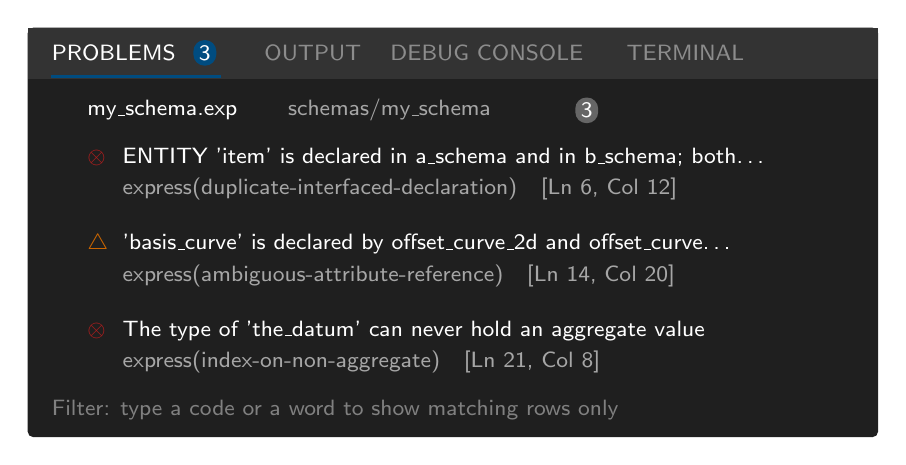
\begin{tikzpicture}[x=1cm,y=1cm,
        txt/.style={font=\footnotesize\sffamily,text=white,anchor=west,inner sep=0pt},
        dim/.style={font=\footnotesize\sffamily,text=black!35,anchor=west,inner sep=0pt},
        tab/.style={font=\footnotesize\sffamily,text=black!45,anchor=west,inner sep=0pt}]
      \fill[black!88,rounded corners=2pt] (0,0) rectangle (10.8,5.2);
      \fill[black!80] (0,4.55) rectangle (10.8,5.2);
      \node[txt,text=white] at (0.3,4.88) {PROBLEMS};
      \node[font=\footnotesize\sffamily,text=white,fill=sc4blue,rounded corners=4pt,inner sep=2pt] at (2.25,4.88) {3};
      \node[tab] at (3.0,4.88) {OUTPUT};
      \node[tab] at (4.6,4.88) {DEBUG CONSOLE};
      \node[tab] at (7.6,4.88) {TERMINAL};
      \draw[sc4blue,line width=1.2pt] (0.3,4.58) -- (2.45,4.58);
      % file row
      \node[txt,text=black!40] at (0.3,4.15) {$\blacktriangledown$};
      \node[txt] at (0.75,4.15) {my\_schema.exp};
      \node[dim] at (3.3,4.15) {schemas/my\_schema};
      \node[font=\footnotesize\sffamily,text=white,fill=black!60,rounded corners=4pt,inner sep=2pt] at (7.1,4.15) {3};
      % problem rows: icon, message; second line: source(code) and position
      \node[txt,text=errred] at (0.75,3.55) {$\otimes$};
      \node[txt] at (1.2,3.55) {ENTITY 'item' is declared in a\_schema and in b\_schema; both\ldots};
      \node[dim] at (1.2,3.15) {express(duplicate-interfaced-declaration)\quad [Ln 6, Col 12]};
      \node[txt,text=orange!80!black] at (0.75,2.45) {$\triangle$};
      \node[txt] at (1.2,2.45) {'basis\_curve' is declared by offset\_curve\_2d and offset\_curve\ldots};
      \node[dim] at (1.2,2.05) {express(ambiguous-attribute-reference)\quad [Ln 14, Col 20]};
      \node[txt,text=errred] at (0.75,1.35) {$\otimes$};
      \node[txt] at (1.2,1.35) {The type of 'the\_datum' can never hold an aggregate value};
      \node[dim] at (1.2,0.95) {express(index-on-non-aggregate)\quad [Ln 21, Col 8]};
      \node[dim,text=black!50] at (0.3,0.35) {Filter: type a code or a word to show matching rows only};
    \end{tikzpicture}%
  }
  \medskip

  \footnotesize
  Open it with \code{Ctrl+Shift+M} (macOS \code{Cmd+Shift+M}). Click a row to jump to the
  line. The filter box narrows the list to one code or one word. Rows with a light bulb
  offer a quick fix, for example for a name in the wrong case.
\end{frame}

%--------------------------------------------------------------------
\begin{frame}{You install it from the VS Code Marketplace}
  \begin{enumerate}
    \item Open VS Code. Press \code{Ctrl+Shift+X} (macOS: \code{Cmd+Shift+X}) to open the Extensions view.
    \item Search for \textbf{EXPRESSsuite}. Click \textbf{Install}.
    \item Open a folder that contains \code{.exp} files, for example a clone of the wg12-step repository.
    \item Open any \code{.exp} file. The extension starts and reads the folder.
  \end{enumerate}
  \medskip
  Works on Windows, macOS and Linux. Needs VS Code 1.140 or newer.
  \medskip

  \footnotesize\color{sc4grey}
  By default, files whose name contains \code{\_lf.exp} or \code{concatenated} are loaded
  but not interpreted: you can open and read them, but they are not checked and their
  names are not indexed. They are generated copies of the module files, and interpreting
  them would duplicate every name. Setting: \code{expresssuite.excludedFiles}.
\end{frame}


\section{The checks provided in the Problems view, with examples}

%--------------------------------------------------------------------
\begin{frame}{Five checks apply clauses of ISO 10303-11:2004}
  \setlength{\tabcolsep}{4pt}
  \begin{tabular}{@{}>{\raggedright\arraybackslash}p{4.2cm}>{\raggedright\arraybackslash}p{1.6cm}>{\raggedright\arraybackslash}p{4.2cm}@{}}
    \toprule
    \textbf{Diagnostic code} & \textbf{Clause} & \textbf{What it reports} \\
    \midrule
    \code{duplicate-interfaced-\newline declaration} & 10.1 b, cl.\ 11 & one name, two declarations in one schema scope \\[2pt]
    \code{ambiguous-attribute-\newline reference}   & 12.7.3 & \code{x.a} where two entities declare \code{a} at the same depth \\[2pt]
    \code{redeclaration-not-\newline specialization} & 9.2.3.4, 9.2.7 & a redeclared attribute widens the original type \\[2pt]
    \code{index-on-non-\newline aggregate}          & 12.6.1 & \code{x[1]} where \code{x} can never be an aggregate \\[2pt]
    \code{reference-statement-\newline missing}     & cl.\ 11 & a name is used but not interfaced \\
    \bottomrule
  \end{tabular}
  \medskip

  A \emph{linking error} is also reported when a name cannot be found at all.
  The next slides show one example of each check.
\end{frame}

%--------------------------------------------------------------------
\begin{frame}{Four checks apply SC4, TF1 and WG11 conventions}
  \setlength{\tabcolsep}{4pt}
  \begin{tabular}{@{}>{\raggedright\arraybackslash}p{4.2cm}>{\raggedright\arraybackslash}p{1.6cm}>{\raggedright\arraybackslash}p{4.2cm}@{}}
    \toprule
    \textbf{Diagnostic code} & \textbf{Source} & \textbf{What it reports} \\
    \midrule
    \code{declaration-name-case}           & SC4 rule & an ARM entity in lowercase, or a MIM name in uppercase; a quick fix is offered \\[2pt]
    \code{duplicate-loop-index}            & 13.9.1 & a \code{LOCAL} variable redeclares a \code{REPEAT} index \\[2pt]
    \code{informal-proposition-*}          & TF1 rule & an \code{IPn} annotation without its \code{--IPn:} signature \\[2pt]
    \code{redundant-declaration}           & WG11 N239 & an identical repeated definition in a long form (warning) \\
    \bottomrule
  \end{tabular}
  \medskip

  These rules are not in ISO 10303-11. They are SC4, TF1 and WG11 conventions, applied while editing.
\end{frame}

%--------------------------------------------------------------------
\begin{frame}[fragile]{One name with two declarations is reported in every schema that sees both}
  Clause 11 defines what a schema \emph{sees}: its own declarations, plus what
  \code{USE FROM} and \code{REFERENCE FROM} bring in. In one scope, a name may
  denote one declaration only (10.1 b).
\begin{lstlisting}
SCHEMA a_schema;  ENTITY item; END_ENTITY;  END_SCHEMA;
SCHEMA b_schema;  ENTITY item; END_ENTITY;  END_SCHEMA;

SCHEMA my_schema;
  USE FROM a_schema;
  USE FROM b_schema;   -- item now arrives twice
END_SCHEMA;
\end{lstlisting}
  \diag{duplicate-interfaced-declaration: ENTITY 'item' is declared in a\_schema and in b\_schema; both are visible in my\_schema}
  \medskip
  The report is placed on the \code{USE FROM} line that brought the second copy.
\end{frame}

%--------------------------------------------------------------------
\begin{frame}[fragile]{An attribute reference looks only in the entity, its supertypes and its subtypes}
  ISO 10303-11:2004 12.7.3: for \code{x.a}, the attribute \code{a} is searched in
  the declared type of \code{x}, then in its supertypes and subtypes, nearest first.
  Never in a sibling entity.
\begin{lstlisting}
ENTITY curve; END_ENTITY;
ENTITY offset_curve_2d SUBTYPE OF (curve);
  basis_curve : curve; END_ENTITY;
ENTITY offset_curve_3d SUBTYPE OF (curve);
  basis_curve : curve; END_ENTITY;

-- somewhere: c : curve;  ...  c.basis_curve
\end{lstlisting}
  \diag{ambiguous-attribute-reference (warning): 'basis\_curve' is declared by offset\_curve\_2d and offset\_curve\_3d at the same depth}
  Write \code{c\textbackslash offset\_curve\_2d.basis\_curve} to say which one you mean.
\end{frame}

%--------------------------------------------------------------------
\begin{frame}[fragile]{A redeclared attribute must keep or narrow the original type}
  ISO 10303-11:2004 9.2.3.4 a) with 9.2.7: the new type shall be the same as, or a
  specialization of, the original type. \code{INTEGER} narrows \code{REAL};
  \code{SET OF x} narrows \code{BAG OF x}; a subtype narrows its supertype.
\begin{lstlisting}
ENTITY measured;
  value : REAL;
END_ENTITY;

ENTITY counted SUBTYPE OF (measured);
  SELF\measured.value : INTEGER;     -- accepted: narrower
END_ENTITY;

ENTITY wrong SUBTYPE OF (measured);
  SELF\measured.value : STRING;      -- reported
END_ENTITY;
\end{lstlisting}
  \diag{redeclaration-not-specialization: STRING is not a specialization of REAL}
\end{frame}

%--------------------------------------------------------------------
\begin{frame}[fragile]{Indexing a value that can never be an aggregate is an error}
  ISO 10303-11:2004 12.6.1: the operand of \code{[ ]} shall be an aggregate value
  (a \code{LIST}, \code{SET}, \code{BAG} or \code{ARRAY}). This slip, taken from a
  draft of ISO 10303-47, was not reported before 0.5.0.
\begin{lstlisting}
ENTITY datum;
  identification : STRING;
END_ENTITY;

ENTITY holder;
  the_datum : datum;          -- one instance, not a list
WHERE
  WR1: the_datum[1]\datum.identification <> 'x';
END_ENTITY;
\end{lstlisting}
  \diag{index-on-non-aggregate: the type of 'the\_datum' can never hold an aggregate value}
\end{frame}

%--------------------------------------------------------------------
\begin{frame}{Letter case follows the SC4 convention: ARM capitalised, MIM lowercase}
  ISO 10303-11 gives letter case no meaning. SC4 schemas do: the ARM entity is
  \code{Product}, the MIM entity is \code{product}, and they are two different
  entities. EXPRESSsuite applies this project rule (rulings of 2026-10-29 and 2026-10-30):
  \begin{itemize}
    \item Entity names and schema names bind only to the exact spelling.
      \code{SUBTYPE OF (mesh)} does not name \code{ENTITY Mesh}.
    \item Type, attribute, function, rule and enumeration names bind regardless of case.
      \code{x : Unit\_kind} names \code{TYPE unit\_kind}.
    \item In a long form (schema name ends in \code{\_lf}) every name binds regardless of case,
      as WG11 N239 requires.
  \end{itemize}
  \medskip
  The published SMRL v8 follows the convention without exception: 3,460 of 3,460 ARM
  entity names begin with an uppercase letter, 1,359 of 1,359 MIM entity names with a lowercase one.
\end{frame}

%--------------------------------------------------------------------
\begin{frame}[fragile]{A MIM reference written in ARM spelling is reported as not found}
  In the published assembly MIM, one \code{DERIVE} line writes the supertype in ARM spelling.
  The 67 other references in the same file are lowercase.
\begin{lstlisting}
ENTITY a3m_equivalence_criterion_for_assembly
  SUBTYPE OF (a3m_equivalence_criterion);
  SELF\a3m_equivalence_criterion.measured_data_type : ...;
DERIVE
  SELF\A3m_equivalence_criterion.accuracy_types : LIST [0:0] OF ...;
END_ENTITY;
\end{lstlisting}
  \diag{The entity 'A3m\_equivalence\_criterion' could not be found in the supertype/subtype of 'a3m\_equivalence\_criterion\_for\_assembly'}
  \medskip
  The fix is one letter. A message that names the case difference is planned
  (see the backup slides).
\end{frame}

%--------------------------------------------------------------------
\begin{frame}{Interfaces follow clause 11: USE FROM passes names on, REFERENCE FROM does not}
  \centering
  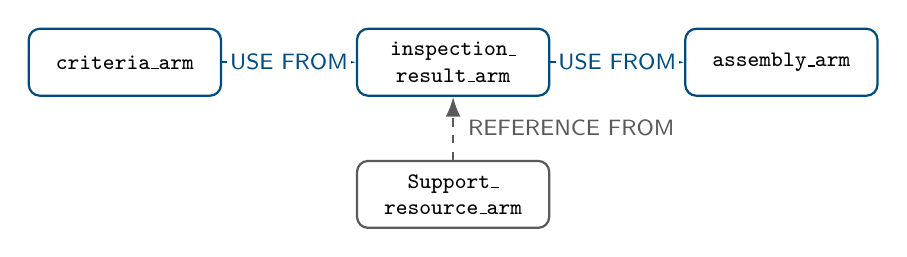
\begin{tikzpicture}[
      box/.style={draw=sc4blue,thick,rounded corners,minimum height=0.85cm,text width=2.3cm,align=center,font=\footnotesize\ttfamily,inner xsep=2pt},
      use/.style={-{Latex[length=2.5mm]},thick,sc4blue},
      ref/.style={-{Latex[length=2.5mm]},thick,sc4grey,dashed},
      lab/.style={font=\footnotesize,fill=white,inner sep=1pt}]
    \node[box] (c) {criteria\_arm};
    \node[box,right=1.7cm of c] (b) {inspection\_\\result\_arm};
    \node[box,right=1.7cm of b] (a) {assembly\_arm};
    \node[box,draw=sc4grey,below=0.8cm of b] (s) {Support\_\\resource\_arm};
    \draw[use] (c) -- node[lab] {USE FROM} (b);
    \draw[use] (b) -- node[lab] {USE FROM} (a);
    \draw[ref] (s) -- node[lab,right=4pt,fill=none] {REFERENCE FROM} (b);
  \end{tikzpicture}
  \medskip
  \begin{itemize}
    \item The assembly ARM sees every declaration of the criteria ARM, two steps away,
      because \code{USE FROM} re-exports what it imports (11.1, 11.3).
    \item The assembly ARM does \emph{not} see \code{Support\_resource\_arm}: a
      \code{REFERENCE FROM} is never passed on (11.2, 11.3).
    \item Item lists and renames are honoured. One declaration reached by two routes counts once.
  \end{itemize}
  \footnotesize\color{sc4grey}Short names: \code{criteria\_arm} is \code{Annotated\_3d\_model\_equivalence\_criteria\_arm}, and so on.
\end{frame}




%--------------------------------------------------------------------
\begin{frame}{Two type properties are proved: specialization and indexability}
  \setlength{\tabcolsep}{4pt}
  \begin{tabular}{@{}>{\raggedright\arraybackslash}p{3.0cm}>{\raggedright\arraybackslash}p{1.9cm}>{\raggedright\arraybackslash}p{5.1cm}@{}}
    \toprule
    \textbf{Check} & \textbf{Clause} & \textbf{What is proved} \\
    \midrule
    redeclared attribute type & 9.2.3.4, 9.2.7 & \code{spec\_sound}: if the relation accepts the new type, every value of the new type is a value of the original type \\[4pt]
    index on a non-aggregate & 12.6.1 & \code{notIndexable\_sound}: if the predicate holds for a type, no value of that type can be indexed, as a binary, a string or an aggregate \\
    \bottomrule
  \end{tabular}
  \medskip

  Both are proved against a transcription of eengine's value semantics
  (\code{TypeP}), so "value" means what the reference validator means by it.
\end{frame}

%--------------------------------------------------------------------
\begin{frame}{Two scope properties are proved: 12.7.3 visibility and clause 11 scope}
  \setlength{\tabcolsep}{3pt}
  \begin{tabular}{@{}>{\raggedright\arraybackslash}p{2.5cm}>{\raggedright\arraybackslash}p{1.8cm}>{\raggedright\arraybackslash}p{5.9cm}@{}}
    \toprule
    \textbf{Check} & \textbf{Clause} & \textbf{What is proved} \\
    \midrule
    reference scope (\code{x.a}, \code{x\textbackslash e}) & 12.7.3, 12.7.4 & \code{mem\_visible\_iff}, \code{resolve\_unique}, \code{resolve\_ambiguous}: the walk finds exactly the 12.7.3 set; ambiguity exactly when two entities at the nearest depth declare the name \\[4pt]
    schema scope and clashes & 10.1 b, cl.\ 11 & \code{iterate\_sound}, \code{export\_complete}, \code{clash\_iff}: the loop computes exactly the clause 11 scope; a clash exactly when one name denotes two declarations \\
    \bottomrule
  \end{tabular}
  \medskip

  \footnotesize\color{sc4grey}
  In Lean, \code{sorry} marks a proof left open. The folder contains none: 78 theorems,
  93 build-checked facts, the three standard axioms only.
\end{frame}


\section{Descriptions, diagrams and formulas}

%--------------------------------------------------------------------
\begin{frame}{Point at a name to read its rendered description}
  SC4 schemas carry their documentation inside the \code{.exp} file, as
  \emph{annotated EXPRESS}: \code{(*"schema.entity" ... *)} blocks after
  \code{END\_SCHEMA}. EXPRESSsuite renders them.
  \begin{itemize}
    \item \textbf{Hover}: move the mouse over a name. A popup shows its description,
      with cross-references as links and formulas as pictures.
    \item \textbf{Show Description} (right-click): the full description opens in a panel
      beside the editor. Click a link in it to open the description of that name.
    \item The description is found through the schema's interfaces, so hovering
      \code{string\_literal} in a schema that references it shows the owning
      schema's text.
  \end{itemize}
  \medskip
  \footnotesize\color{sc4grey}
  Formulas written as \code{stem:[...]} (AsciiMath) or \code{latexmath:[...]} are typeset
  by Plurimath, the same converter Metanorma uses to publish the standards.
\end{frame}

%--------------------------------------------------------------------
\begin{frame}{EXPRESS-G diagrams open from the schema and link back to the source}
  \begin{itemize}
    \item \textbf{Show EXPRESS-G Diagram} (right-click): opens the \code{expgN.svg}
      diagram that contains the entity at the cursor. If several diagrams match, a list is offered.
    \item Click any box in the diagram. The editor jumps to that entity's declaration.
    \item \textbf{Detect Duplicate Declarations in Schema Closure}: the same clause 11
      check as the live diagnostic, on demand, for the schema at the cursor.
  \end{itemize}
\end{frame}

%--------------------------------------------------------------------
\begin{frame}{Write a formula in the playground, check it, then insert it into the schema}
  \centering
  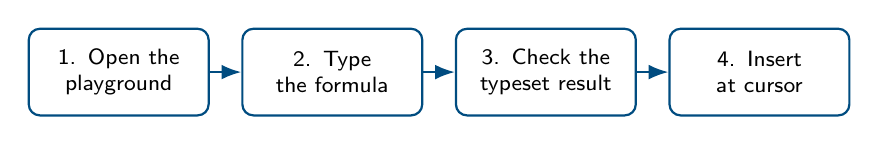
\begin{tikzpicture}[
      wfstep/.style={draw=sc4blue,thick,rounded corners,minimum height=1.1cm,text width=2.05cm,align=center,font=\footnotesize},
      next/.style={-{Latex[length=2.5mm]},thick,sc4blue}]
    \node[wfstep] (s1) {1. Open the playground};
    \node[wfstep,right=0.4cm of s1] (s2) {2. Type the formula};
    \node[wfstep,right=0.4cm of s2] (s3) {3. Check the typeset result};
    \node[wfstep,right=0.4cm of s3] (s4) {4. Insert at cursor};
    \draw[next] (s1) -- (s2); \draw[next] (s2) -- (s3); \draw[next] (s3) -- (s4);
  \end{tikzpicture}
  \medskip
  \begin{enumerate}
    \item Command Palette (\code{Ctrl+Shift+P}, macOS \code{Cmd+Shift+P}):
      \textbf{EXPRESSsuite: Open AsciiMath Playground}. A panel with two panes opens.
    \item Type AsciiMath in the left pane, for example \code{sum\_(i=1)\^{}n i\^{}3}.
    \item The right pane shows the formula typeset. It updates when you stop typing.
    \item Place the cursor in the description in the editor, then click
      \textbf{Insert at cursor}. The playground writes \code{stem:[...]} there.
  \end{enumerate}
  \medskip
  \footnotesize\color{sc4grey}
  The other direction: select an existing \code{stem:[...]} in the editor, right-click,
  \textbf{Send Selection to AsciiMath Playground}, and edit it there.
\end{frame}




\section{Confidential schema content}

%--------------------------------------------------------------------
\begin{frame}{EXPRESSsuite itself sends nothing anywhere}
  \begin{itemize}
    \item The extension makes \textbf{no network calls}. There is no telemetry, no update check,
      no download at run time.
    \item Every panel (description, diagram, playground) is configured with the browser rule
      \code{connect-src 'none'}, so a panel cannot open a connection even if it tried.
    \item The source code contains no \code{fetch} and no \code{http} import. You can check
      this yourself: the code is public.
    \item All rendering, including formulas, runs on your computer.
  \end{itemize}
  \medskip
  This matters for schemas under development that are not yet public.
\end{frame}

%--------------------------------------------------------------------
\begin{frame}{VS Code itself ships GitHub Copilot Chat, which does send text out}
  Copilot Chat is built into VS Code. Its right-click entries (\emph{Explain},
  \emph{Add File to Chat}, \emph{Open Inline Chat}, \emph{Review}) send the selected
  text, the surrounding lines and parts of other open files to Microsoft.
  Starting VS Code with \code{--disable-extensions} does not remove them.
  \medskip

  For schemas under non-disclosure, do one of these:
  \begin{enumerate}
    \item Sign out of GitHub in that VS Code window (account icon, bottom left).
      Without a login, Copilot Chat cannot reach its service.
    \item Or set \code{"chat.disableAIFeatures": true} in the workspace settings file
      \code{.vscode/settings.json}.
    \item Best practice: keep one separate, signed-out VS Code window for confidential schemas.
  \end{enumerate}
\end{frame}

\section{Where to get it, and where to report a problem}

%--------------------------------------------------------------------
\begin{frame}{Where to get it, and where to report a problem}
  \begin{itemize}
    \item Marketplace: search \textbf{EXPRESSsuite} in VS Code, or open\\
      \code{marketplace.visualstudio.com/items?}\\
      \code{itemName=TRThurman.expresssuite}
    \item Source, release notes and issues:\\
      \code{github.com/TRThurman/EXPRESSsuite}
    \item To report a problem: open an issue with the schema text that shows it and the
      message from the Problems view. The issue form asks for both.
    \item Licence: derived from NIST easyEXPRESS (Sylvere Krima, Allison Barnard Feeney,
      Rosemary Astheimer). NIST software is public domain in the United States.
      Modifications are listed in \code{NOTICE.md}.
  \end{itemize}
  \vfill
  \centering\footnotesize\color{sc4grey}
  Thomas Thurman, \code{thomas@trthurman.consulting}
\end{frame}

\AtBeginSection{}
\section*{Backup: tool maintenance}
\begin{frame}
  \vfill\centering
  {\footnotesize\color{sc4grey}Backup}\\[0.6em]
  {\Large\bfseries\color{sc4blue}Tool maintenance}\\[0.8em]
  {\normalsize how every change is tested, and the known limits of 0.5.0}
  \vfill
\end{frame}

%--------------------------------------------------------------------
\begin{frame}{Every change is tested against the 1,410 published SMRL v8 schema files}
  \centering
  \begin{tabular}{@{}c@{\hspace{0.5cm}}c@{\hspace{0.5cm}}c@{}}
    {\huge\color{sc4blue}1,410} & {\huge\color{sc4blue}1,287} & {\huge\color{sc4blue}103} \\
    \footnotesize \code{.exp} files & \footnotesize loaded as one workspace & \footnotesize long forms, built alone \\
  \end{tabular}
  \medskip

  \begin{itemize}
    \item Every diagnostic on every file is recorded in a baseline file in the repository.
    \item A code change that moves one diagnostic shows up as a reviewable difference.
    \item The same result is produced on macOS, Linux and Windows, and on repeated runs
      in one process.
    \item The baseline records behaviour, not correctness. Known false positives are listed
      next to it, so they are not mistaken for schema defects.
  \end{itemize}
\end{frame}

%--------------------------------------------------------------------
\begin{frame}{Known limits in 0.5.0}
  \begin{itemize}
    \item Long forms and concatenated files are loaded but not interpreted by default.
      Interpreted together with the modules, they would duplicate every name.
    \item Some attribute references inside \code{QUERY} expressions, function results and
      long attribute paths are not typed yet. They are reported as linking errors.
      These sites are listed with the baseline as known false positives.
    \item The letter-case rule is stricter than ISO 10303-11. A reference written in
      the wrong case is reported as "could not be found". A clearer message is planned.
    \item The EXPRESS-G viewer needs the \code{expgN.svg} files beside the schema,
      as wg12-step provides them.
  \end{itemize}
\end{frame}

%--------------------------------------------------------------------
\begin{frame}{EXPRESSsuite uses Lean 4 the way AWS uses it for Cedar: an executable model that the code must match}
  \begin{itemize}
    \item Lean 4 is a programming language and a proof assistant in one. A definition
      written in Lean runs, and a theorem about it is checked line by line by a small
      kernel, the only part that has to be trusted.
    \item AWS builds its Cedar authorization language this way: the model of each component
      is written in Lean, its properties are proved, the product is written in Rust, and
      no version is released unless the model, the proofs and the tests that compare the
      two are current. The models are about ten times smaller than the product.
  \end{itemize}
  \medskip
  \footnotesize\color{sc4grey}
  Sources: AWS Open Source Blog, ``Lean Into Verified Software Development'', 2024;
  lean-lang.org/use-cases/cedar. Full list on the ``Lean sources'' slide.
\end{frame}

%--------------------------------------------------------------------
\begin{frame}{Four of the nine checks are built from an executable Lean 4 model that the code must match}
  The method is the one AWS uses for its Cedar language (previous slide). The four checks
  are those whose code holds 81\,\% of the decision points of all nine (McCabe cyclomatic
  complexity; the table is on the next slide).
  \begin{itemize}
    \item \textbf{Model:} the clause semantics of each check are written in Lean and proved:
      the specialization relation (9.2.3.4), the indexability predicate (12.6.1), the
      12.7.3 visibility walk, and the clause 11 scope with its clashes (10.1 b).
    \item \textbf{Product:} the TypeScript checker transcribes those definitions clause by
      clause and cites each one at the function that implements it.
    \item \textbf{Agreement:} the standard's own examples are build-checked facts in Lean,
      the unit tests exercise the same cases in TypeScript, and the SMRL v8 baseline
      pins the result on 1,390 published schemas.
  \end{itemize}
\end{frame}


%--------------------------------------------------------------------
\begin{frame}{The four proved checks hold 81\,\% of the decision points of all nine checks}
  \footnotesize
  \setlength{\tabcolsep}{4pt}
  \begin{tabular}{@{}>{\raggedright\arraybackslash}p{6.6cm}>{\raggedright\arraybackslash}p{1.7cm}r@{}}
    \toprule
    \textbf{Check} & \textbf{Lean proof} & \textbf{Complexity} \\
    \midrule
    redeclaration-not-specialization & yes & 157 \\
    duplicate-interfaced-declaration (and redundant-declaration) & yes & 139 \\
    index-on-non-aggregate & yes & 138 \\
    informal-proposition-* & no & 54 \\
    reference-statement-missing & no & 30 \\
    ambiguous-attribute-reference & yes & 15 \\
    declaration-name-case & no & 14 \\
    duplicate-loop-index & no & 7 \\
    \midrule
    proved checks & & 449 of 554 \\
    \bottomrule
  \end{tabular}
  \medskip

  \color{sc4grey}
  McCabe cyclomatic complexity per check: its validator method plus the module that
  implements its relation, measured with ESLint's \code{complexity} rule on 0.5.0. The
  resolved-type builder (216) serves the two type checks and is split between them.
\end{frame}

%--------------------------------------------------------------------
\begin{frame}{Where the model lives, and what it does not cover}
  \begin{itemize}
    \item The folder \code{lean/} in the repository holds the definitions of the four checks
      and the proofs about them. \code{lake build} checks every proof; it is run by hand,
      not yet by the extension's continuous integration.
    \item The TypeScript code of the checker is a line-by-line transcription of those
      definitions, kept in step with them.
    \item The standard's own examples (9.2.3.4 EXAMPLE 2 and 3, 11.3 EXAMPLE 2) are
      build-checked facts.
    \item Two mistakes in the first version of the redeclaration rule were found by
      these examples, not by users: \code{SET OF x} narrows \code{BAG OF x}, and
      \code{INTEGER} narrows \code{REAL} (9.2.7).
    \item The other five checks (name case, loop index, informal propositions, missing
      reference statements, redundant repeats) are tested, not proved.
  \end{itemize}
\end{frame}

\section*{Lean sources}
\begin{frame}{Lean sources}
  \footnotesize
  \begin{itemize}
    \setlength{\itemsep}{0.3em}
    \item K. Hietala, E. Torlak, ``Lean Into Verified Software Development'', AWS Open Source
      Blog, 8 April 2024. \code{aws.amazon.com/blogs/opensource/}\\
      \code{lean-into-verified-software-development/}
    \item ``Lean Powers Secure Software at AWS: Cedar's Journey with Verified Development'',
      \code{lean-lang.org/use-cases/cedar/}
    \item J. W. Cutler et al., ``Cedar: A New Language for Expressive, Fast, Safe, and
      Analyzable Authorization'', arXiv:2403.04651, 2024.
    \item Cedar security documentation, \code{docs.cedarpolicy.com/other/security.html}
    \item M. de Medeiros et al., ``Verified Foundations for Differential Privacy'' (SampCert),
      arXiv:2412.01671, 2024. \code{reservoir.lean-lang.org/@leanprover/sampcert}
    \item ``Scaling Verification of Cryptographic Software with Aeneas, Rust, and Lean'',
      arXiv:2609.15648, 2026; Microsoft Research, ``Verifying Rust cryptography in SymCrypt,
      from standards to code''.
    \item Galois, ``Real-time Robotics Control in the Lean Language'', 29 March 2021.
    \item Lean homepage and use cases, \code{lean-lang.org}; Software Verification in Lean
      workshop, 2026.
  \end{itemize}
\end{frame}

\end{document}
